\section{Experiments and results}
\label{sec:results}

\subsection{Baseline}
On all 1,078 development notes, logistic regression chooses $C=100$, almost no regularisation, and reaches a 5-fold CV error of \LRcv{} $\pm$ \LRcvse{}: 6 wrong notes. Nested CV, which also accounts for choosing $C$, gives \LRnested{} $\pm$ \LRnestedse{} (Appendix~\ref{app:baseline}). The majority-class rule errs on 45.3\%. Even without regularisation, logistic regression still gets 4 of its own training notes wrong, so the classes are not linearly separable in these features. The baseline's remaining error is therefore bias, not a lack of data, and that already predicts how its learning curve will look.

\subsection{Learning curves}
\label{sec:curves}
\begin{figure}[t]
  \centering
  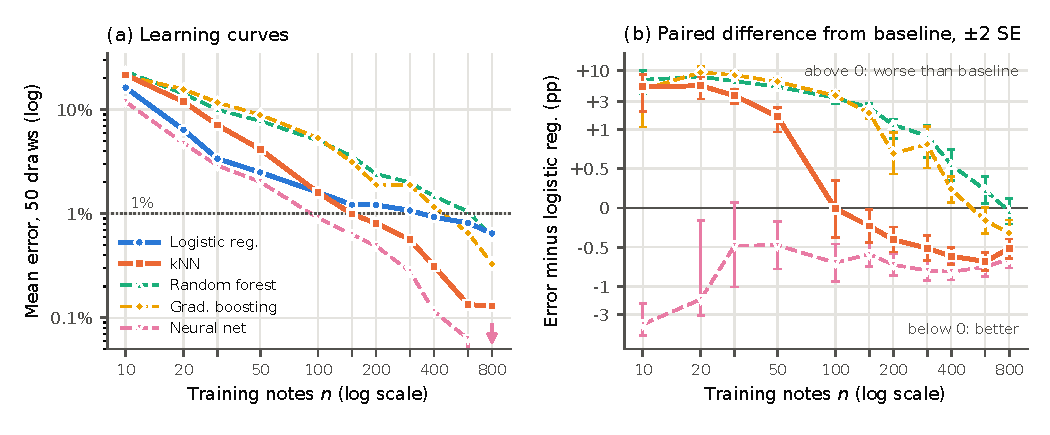
\includegraphics[width=\linewidth]{../figures/learning_curves.pdf}
  \caption{(a) Mean error on held-out development notes over 50 draws per size (log--log). Solid lines are the core methods, dashed lines the later-course extensions. The arrow marks the neural network at $n=800$, where all 50 draws had zero errors. (b) Paired difference from logistic regression on the same draws, in percentage points, with $\pm$2 SE bars (symmetric-log axis, linear between $-1$ and $+1$). Below 0 is better than the baseline.}
  \label{fig:curves}
\end{figure}

Figure~\ref{fig:curves} shows the main result; full numbers are in Appendix~\ref{app:full}.

\paragraph{Logistic regression vs.\ $k$NN.} Logistic regression is clearly better at small sizes: at 50 notes it errs on \errLRFifty{} against \errKNNFifty{} for $k$NN, a paired gap of \diffKNNFifty{} $\pm$ \seKNNFifty{} points. The two tie at 100 notes (\errLRHundred{} vs.\ \errKNNHundred{}). From 150 notes $k$NN is clearly better (\diffKNNOneFifty{} $\pm$ \seKNNOneFifty{} points) and the gap keeps growing, because logistic regression flattens out while $k$NN does not: at 800 notes the errors are \errLREightHundred{} and \errKNNEightHundred{}, and $k$NN wins \winsKNNEightHundred{} of 50 draws. Inner CV picks $k=1$ in most draws at every size (Table~\ref{tab:params}). This matches the crossing curves Perlich et al.\ \cite{perlich2003tree} report for logistic regression against a more flexible learner, which has the lower error at large sizes but needs more data to get there.

\paragraph{Extensions.} The two tree ensembles are worse than the baseline at every size up to 400 notes, often by several points: at 100 notes the forest errs on \errRFHundred{} and boosting on \errGBHundred{}. Boosting is clearly better than the baseline only at 800 notes (\errGBEightHundred{}), and the forest only ties it there. A larger forest grid on all development notes does not help (Appendix~\ref{app:forest}), so this is not a tuning problem. The small neural network, in contrast, has the lowest mean error of all five methods at every size. At 10 notes it errs on \errNNTen{} against \errLRTen{} for the baseline (\diffNNTen{} $\pm$ \seNNTen{} points), and at 800 notes none of its 50 draws makes a single error. CV most often picks the 8-unit network with weak weight decay.

\begin{figure}[t]
  \begin{minipage}[b]{0.44\linewidth}
    \centering
    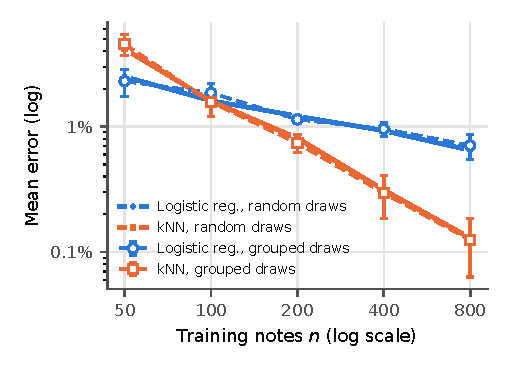
\includegraphics[width=\linewidth]{../figures/grouped.pdf}
    \captionof{figure}{Random draws (solid) vs.\ draws that keep each 8-row pseudo-specimen on one side of every split (dashed, $\pm$2 SE).}
    \label{fig:grouped}
  \end{minipage}\hfill
  \begin{minipage}[b]{0.53\linewidth}
    \centering
    \captionof{table}{Training notes needed for the mean error to reach 2\% and 1\%, interpolated on the learning curves, with bootstrap 95\% intervals over draws. $^\dagger$Extension.}
    \label{tab:reach}
    \small
    \setlength{\tabcolsep}{4pt}
    % generated by src/make_tables.py
\begin{tabular}{lrcrc}
\toprule
Method & \multicolumn{2}{c}{2\% error} & \multicolumn{2}{c}{1\% error} \\
 & $n$ & 95\% CI & $n$ & 95\% CI \\
\midrule
Logistic regression & 71 & 58--83 & 345 & 278--415 \\
$k$NN & 85 & 77--95 & 149 & 131--176 \\
Random forest$^\dagger$ & 297 & 247--326 & 614 & 560--648 \\
Gradient boosting$^\dagger$ & 195 & 184--304 & 446 & 403--479 \\
Neural network$^\dagger$ & 50 & 41--58 & 92 & 80--108 \\
\bottomrule
\end{tabular}

    \vspace{14pt}
  \end{minipage}
\end{figure}

\paragraph{Notes needed to reach a target.} Table~\ref{tab:reach} turns the curves into the quantity a practitioner would ask for. To reach 2\% error, the neural network needs about \reachNNTwo{} notes and logistic regression \reachLRTwo{}, with $k$NN close behind at \reachKNNTwo{}. To reach 1\%, the order changes: the neural network needs about \reachNNOne{}, $k$NN \reachKNNOne{}, and logistic regression \reachLROne{}, more than twice as many as $k$NN. The forest needs the most at both targets. The bootstrap intervals for the core methods do not overlap at 1\%.

\subsection{Several images per specimen}
\label{sec:grouped}
If $k$NN with $k=1$ wins only because it finds a near-copy of the same physical note in the training set, its advantage should shrink when whole pseudo-specimens are kept on one side of the split. It does not (Figure~\ref{fig:grouped}, Table~\ref{tab:grouped}). With grouped draws, $k$NN errs on \gerrKNNTwoHundred{} at 200 notes and \gerrKNNEightHundred{} at 800, against \errKNNTwoHundred{} and \errKNNEightHundred{} with random draws; logistic regression moves from \errLREightHundred{} to \gerrLREightHundred{} at 800. Grouped 5-fold CV on all development notes gives the same picture (Section~\ref{sec:data}; logistic regression 0.65\% and $k$NN 0.09\% in both cases). Within the limits of our heuristic grouping, the crossover is not an artefact of specimen leakage.

\subsection{Held-out test set}
\label{sec:test}
\begin{table}[t]
  \centering
  \caption{One-time evaluation on the 270 test notes (122 forged), after tuning by 5-fold CV on all development notes. ``Missed'' are forged notes called genuine, ``False al.'' genuine notes called forged. The interval is a Wilson 95\% interval; $p$ is an exact McNemar test against logistic regression. $^\dagger$Extension.}
  \label{tab:test}
  \small
  \setlength{\tabcolsep}{4.5pt}
  % generated by src/make_tables.py
\begin{tabular}{lrrrcrrcr}
\toprule
Method & Dev CV (\%) & Errors & Test (\%) & 95\% CI & Missed & False al. & AUC & $p$ vs LR \\
\midrule
Logistic regression & 0.56 & 1/270 & 0.37 & 0.1--2.1 & 0 & 1 & 0.9999 & -- \\
$k$NN & 0.09 & 1/270 & 0.37 & 0.1--2.1 & 0 & 1 & 0.9966 & 1.00 \\
Random forest$^\dagger$ & 0.56 & 3/270 & 1.11 & 0.4--3.2 & 0 & 3 & 0.9998 & 0.62 \\
Gradient boosting$^\dagger$ & 0.28 & 1/270 & 0.37 & 0.1--2.1 & 0 & 1 & 0.9999 & 1.00 \\
Neural network$^\dagger$ & 0.00 & 0/270 & 0.00 & 0.0--1.4 & 0 & 0 & 1.0000 & 1.00 \\
\bottomrule
\end{tabular}

\end{table}

Table~\ref{tab:test} gives the result of the single test evaluation. Logistic regression, $k$NN and boosting each misclassify \testerrLR{} of 270 notes (\testLR{}), the forest \testerrRF{}, and the neural network none. Every error is a false alarm; no method misses a forgery. These counts are too small to rank the methods: the 95\% intervals overlap heavily, and no McNemar test against the baseline comes close to significance ($p\ge0.62$). This is the outcome we expected before running it, and it is why the learning curves, not the test set, carry our conclusions. ROC curves are in Appendix~\ref{app:roc}.
